\documentclass[
	a4paper, % Paper size, use either a4paper or letterpaper
	10pt, % Default font size, can also use 11pt or 12pt, although this is not recommended
	unnumberedsections, % Comment to enable section numbering
	twoside, % Two side traditional mode where headers and footers change between odd and even pages, comment this option to make them fixed
]{LTJournalArticle}

\addbibresource{refs.bib} % BibLaTeX bibliography file

% A shortened article title to appear in the running head, leave this command empty for no running head

% \footertext{\textit{Journal of Biological Sampling} (2024) 12:533-684} % Text to appear in the footer, leave this command empty for no footer text

\setcounter{page}{1} % The page number of the first page, set this to a higher number if the article is to be part of an issue or larger work

%----------------------------------------------------------------------------------------
%	TITLE SECTION
%----------------------------------------------------------------------------------------

\title{Probabilistic Approaches to 
\\ Energy Conservation in CDNs} % Article title, use manual lines breaks (\\) to beautify the layout

% Authors are listed in a comma-separated list with superscript numbers indicating affiliations
% \thanks{} is used for any text that should be placed in a footnote on the first page, such as the corresponding author's email, journal acceptance dates, a copyright/license notice, keywords, etc
\author{%
	Adarsh Hiremath, Artemas Radik, Andrew Palacci \\
	CS 262: Introduction to Distributed Systems \\
}


%----------------------------------------------------------------------------------------

\begin{document}

\maketitle % Output the title section

%----------------------------------------------------------------------------------------
%	ARTICLE CONTENTS
%----------------------------------------------------------------------------------------

\section{1. Introduction}
% motivation: “we sought to find an application of the replication that we learned that went beyond fault-tolerance, and provided additional benefits to the companies or individuals implementing them. with this project, these benefits are twofold — we show that companies implementing CDNs for content delivery are not only able to deliver content faster (the primary goal) but also more energy-efficiently. in a time where the climate is clearly becoming more at risk and legislation is also beginning to respond, we decided that CDNs were a great place to make advances as to their energy efficiency”
% brief explanation of what CDNs are and what they are typically used for
% the novel contributions of this paper are: A. fitting to different distributions B. new probability calculations C. a way to calculate

\section{2. Existing Methods}

Several recent papers cover the topic of energy consumption in CDNs. Paper \cite{ulIslam2012} proposes a new energy consumption model for CDN surrogates, compares Uniform and Zipfian client redirection policies, and simulates results via a CDNSim testbed \cite{cdnsim}. Critically, the model introduced in \cite{ulIslam2012} does not incorporate network synchronization or transmission costs into it's energy model, opting to instead dismiss them. 

Paper \cite{osmanthesis} does account for costs such as that of transmission energy, but also has a general focus on determining optimal CDN cache sizes (both fixed and variable) via a proposed mixed-integer linear programming model. Notably, \cite{osmanthesis} does not have an apparent focus on optimizing CDN surrogate quantities at scale.

Unlike \cite{osmanthesis} and \cite{ulIslam2012}, paper \cite{biancoCDNs2017} assumes that CDN cache sizes are a constant factor of the primary in order to analyze transmission, synchronization, and other costs in-depth. We were able to closely replicate the findings of \cite{biancoCDNs2017}, with small quantitative differences but identical qualitative conclusions. Their model — which is the basis for our proposed model — aligns closely with the reality of the internet. As a result, it's key to understand their approach, which is outlined in the remainder of this section.

\subsection{2.1. Network Topology}

We represent a CDN as a \textit{primary} server, storing the entire data set, connected to several \textit{surrogate} servers, each of which store a fixed-size subset of the primary's contents. The idea is that surrogates sit on the network edge, closer to end users — minimizing cost, latency, and energy usage. 

Both the primary and surrogates sit in the internet, which at large can be modeled as a three-tier network of ISPs (Internet Service Providers). Each tier can be described as follows:
\begin{enumerate}
    \item Tier one ISPs have global reach and are at the top of the hierarchy.
    \item Tier two ISPs are typically regional or country-based, and are responsible for connecting between tier one and tier three ISPs.
    \item Tier three ISPs provide internet connectivity to end users.
\end{enumerate}



% Efficiently caching content is crucial for highly performant CDNs. Web multimedia data such as text, video, and audio can be exceptionally large, making cache policies essential for ensuring that clients receive data quickly without overburdening the surrogate servers in the CDN. In a simple 3-tier CDN model, we want to move the most popular content to the surrogate servers in the furthest edge of the network - in this case, the 3rd tier.  

% \begin{figure}[h]
% 	\begin{center}
% 		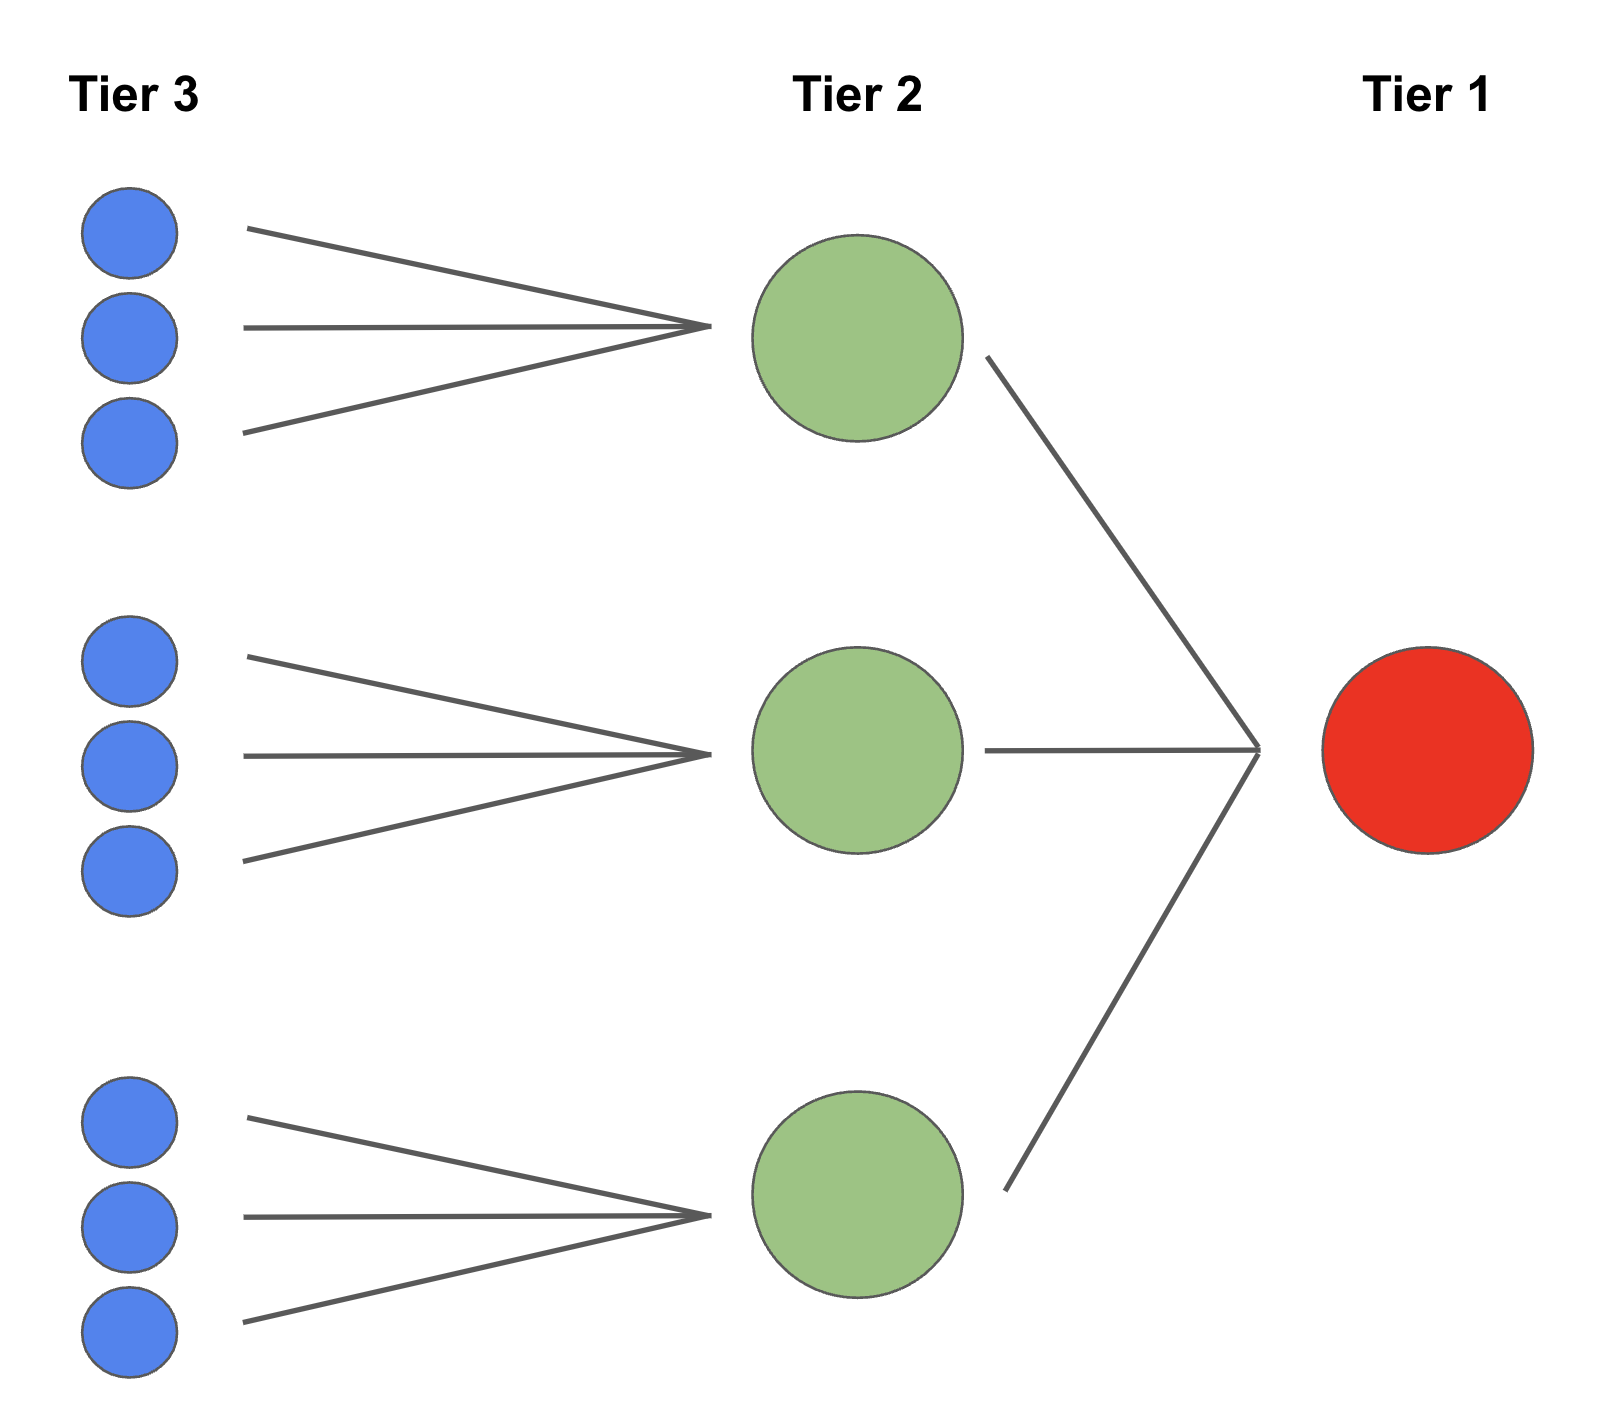
\includegraphics[width=8.1cm]{tier.png}
% 	\end{center}
% 	\caption{A caption for this image.}	
% \end{figure}

% Throughout the paper, we reference the above $3$-tier model. We note the following assumptions and notations about the model: 
% \begin{itemize}
% 	\item Each node in the above model is an ISP. The surrogate servers are placed \textit{within} a tier 3 ISP.
% 	\item The primary server contains all of the content in the CDN, and propagates modified/new content to surrogates according to the cache policy. 
% 	\item There are $T_1$ ISPs in tier $1$, $T_2$ ISPs in tier $2$, and $T_3$ ISPs in tier $3$. 
% 	\item There are $S$ surrogate servers. 
% 	\item $g_3$ represents a group of Tier $3$ ISPs. 
% 	\item The hit probability for each surrogate server is represented as $P_{hit}$.  
	
% \end{itemize}

\subsection{2.2. Cache Policies}

A naive approach to caching content on surrogate servers could be a cache-everywhere policy. In this web caching framework, a cache miss results in a chain of requests upstream to surrogate servers in order to retreive the uncached object. Once the object is found in a server's cache, the object is cached at every intermediate server between the server at the furthest edge of the network and the destination server. Cache-everywhere is observed in many older caching solutions, such as the open-source Harvest/Squid system. 

However, since every server between the edge of the network and the destination server is burdened with a new cached object in the event of a miss, this caching policy is highly inefficent. This policy is usually only employed with smaller objects under 1 kilobyte in size such as HTML pages or CSS stylesheets. Thus, cache-everywhere fails for longer forms of multimedia such as audio and video. 


Another approach is to distribute cached content evenly across all surrogate servers in the network, regardless of how popular the content is. This is done by caching content uniformly. 

Although this policy ensures that all surrogate servers have a similar workload, it is not very effective because it does not consider the popularity of content. This means that highly popular content may still be located far from the furthest edge of the network, and less popular content may be replicated unnecessarily near the edge. This can lead to higher latency and longer initial response times for end clients. Thus, a uniform caching policy should be avoided in high-traffic CDNs. 


The most recent research on green CDNs claims that the Zipf distribution is an optimal choice for determining how to cache data since it takes the popularity of the content into account, unlike the uniform distribution.

The probability mass function (PMF) of the Zipf distribution can be mathematically expressed as:

\[
	P(X=k) = \frac{1/k^{\alpha}}{\zeta(\alpha)}
\] 

where $X$ is a random variable representing the rank of a term in a corpus, $k$ is an integer representing the rank of the term, and $\alpha$ is a parameter that controls the skewness of the distribution. $\zeta(\alpha)$ is the Riemann zeta function, defined by:

\[
	\zeta(\alpha) = \sum{k=1}^{\infty} \frac{1}{k^{\alpha}} 
\] 

Put more simply, Zipf's law states that the $k$th most popular data object will be accessed with probability $\frac{1}{k}$. A cache policy using Zipf's law would allocate cache space to surrogates based on the probability outputted by the PMF of the Zipf distribution. By taking into account the popularity of content using the Zipf distribution with parameter $\alpha = 0.8$, recent research claims that allocating cache by Zipf's law minimizes cache misses. 

\begin{figure}[h]
	\begin{center}
		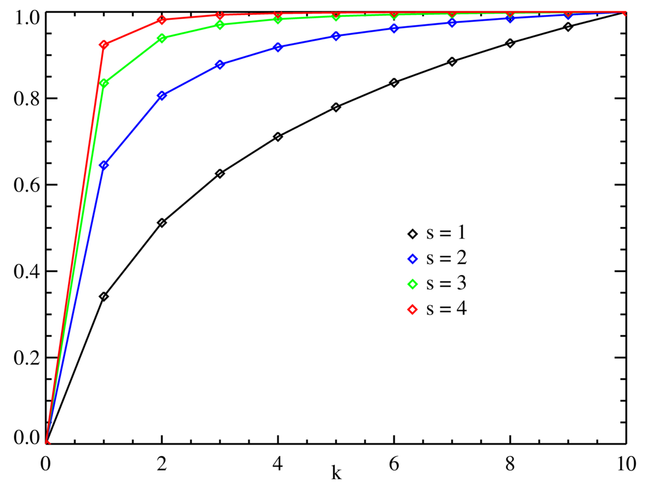
\includegraphics[width=8.1cm]{zipf.png}
	\end{center}
	\caption{A graph of the Zipf distribution CDF for $10$ elements. The horizontal axis is the $k$ parameter.}	
\end{figure}

The graph of the cumulative distribution function (CDF) of the Zipf distribution shows that the top ranked item is overweighted because the rank of each item in the Zipf distribution decreases as the rank of the item increases. This means that the probability of accessing the top-ranked item is much higher than the probability of accessing any other item. 



\subsection{2.3  Calculating a Hit Probability}

\subsection{2.4  Modeling Energy Consumption}

\subsection{2.5  Results}


\section{3. A Better Cache Policy}

While \cite{biancoCDNs2017} asserts that Zipf with $\alpha = 0.8$ is an accurate caching policy for a variety of multimedia, content distributions on modern platforms like Tik Tok, Spotify, and YouTube indicate that alternate distributions could offer a better framework for CDN caching. 

Since platforms like Tik Tok, Spotify, and YouTube typically contain more items with high popularity and more items that spontaneously change in popularity by going viral alright, the distribution of popularity is less skewed than Zipf with $\alpha = 0.8$ might suggest. Therefore, using the Zipf distribution to determine cache allocation especially for short-form video content may not be as effective as for other types of multimedia. Additionally, since short-form video content requires larger amounts of storage space, efficient cache allocation modeling is even more crucial to ensure optimal performance of a CDN.


\subsection{3.1 Pareto Distribution}

We claim that the Pareto distribution is a better alternative to allocating cache space than Zipf with $\alpha = 0.8$. The Pareto principle, also known as the $80/20$ rule, dictates that 20\% of the content is responsible for 80\% of the views. This is  a better model for short-form video content like Tik Tok, which is known for having viral videos that accumulate a large number of views in a short period of time. Allocating more cache space to the most popular 20\% of content using the Pareto distribution could potentially help improve the performance of a CDN for short-form video content.

The probability mass function (PMF) of the Pareto distribution can be mathematically expressed as:

\[
    P(X \geq x) = \left(\frac{x_m}{x}\right)^\alpha
\]

where $X$ is a random variable representing the size of a file, $x$ is the threshold size for caching, $x_m$ is the minimum file size for caching, and $\alpha$ is a parameter that controls the skewness of the distribution. Like the Zipf distribution, the Pareto distribution is a power law distribution, meaning that the ratio of frequencies of any two elements in the distribution is independent of the elements' actual values.  

\begin{figure}[h]
	\begin{center}
		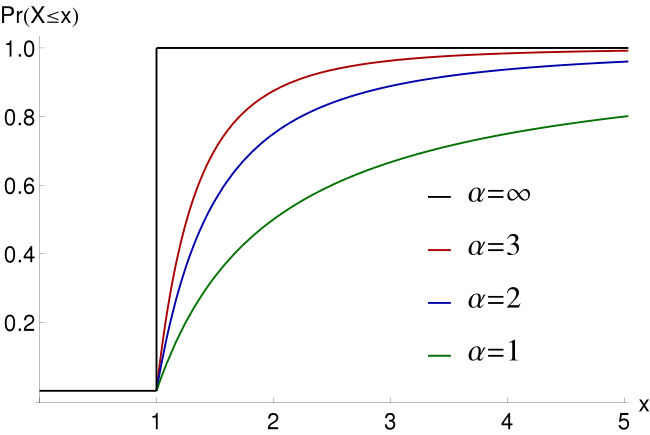
\includegraphics[width=8.1cm]{pareto.png}
	\end{center}
	\caption{A graph of the Pareto distribution CDF for various $\alpha$ with a scale parameter of $1$.}	
\end{figure}

The graph of the cumulative distribution function (CDF) of the Pareto distribution very strongly mirrors the Zipf distribution, which is to be expected because both distributions are monotonically decreasing and positively skewed. However, unlike Zipf, the Pareto distribution indicates that it takes more data objects to reach 80\% of total views. As explained in $3.3$, this addresses the primary concern with using Zipf's law to model modern multimedia. 

\subsection{3.2 Calculating Hit Probability}
\subsection{3.3 Pareto-based Energy Consumption (RESULTS)}

\section{4. Adaptations to Larger CDNs}
So far, the CDN energy consumption model we reference has been very useful for observing how to seek greener content delivery, alongside how using various cache policies affects energy usage. However, while working with the model, we also found some of our original assumptions and constraints to be unintuitive. In this section, we first examine the constraint on the amount of surrogates in our model, and then examine an important missing factor in our energy consumption calculations.

\subsection{4.1 Relaxing Surrogate Constraints}
For one, our above model makes the assumption that $S < T_2$ --- that there are fewer CDN surrogate servers than Tier 2 ISPs, and furthermore that there exists at most one surrogate per Tier 2 ISP. Reminding ourselves that in a realistic Internet hierarchy, Tier 2 ISPs are regional and national providers that operate both closer to clients than Tier 1 ISPs but further than Tier 3 ISPs, this assumption is unrealistic. If a large provider (e.g. TikTok or Spotify) wanted to rapidly deliver content, it would obviously want to have surrogates at as many Tier 3 ISPs as possible, regardless of whether they are connected to the same Tier 2 ISP. 

Furthermore, recalling our goal of optimizing CDN energy consumption, the results we found in previous sections seem to illustrate that adding surrogate servers consistently contributes to decreased normalized energy consumption. We realized this clearly couldn't be true, both in our model and in reality --- once there exists a surrogate in each Tier 3 ISP, there is no way to lower the amount of hops from a client to a surrogate. The only potential benefit of having several surrogates in a single Tier 3 ISP is redundancy, which we do not seek here because surrogates only contain part of the existing content, and our primary server is assumed to be stable. 

Given these two findings, we sought a way to update our constraint such that $S \leq T_3$ instead --- this follows from the fact that it could potentially be useful, and even energy-efficient, to continue adding surrogates until there is a surrogate at each Tier 3 ISP. As a result, we restructured our transmission energy consumption in order to allow for this new constraint. Namely, the probabilities $P_A, P_B, P_C$ of a client's closest hit being at a Tier 3, 2, or 1 ISP must be changed accordingly. 

For the purpose of interpretability, we shall assume that new surrogates will be uniformly randomly assigned to a Tier 3 ISP. Of course, this is not an entirely accurate assumption to make, since some Tier 3 ISPs have far higher priority than others, such as ones in more in-demand geographic areas (New York instead of Montana) or ones with a greater service population. However, our model already makes similar implicit assumptions, such as the fact that clients and surrogates are evenly geographically distributed. Furthermore, our model focuses on differentiating costs \textit{between} ISP tiers, and not \textit{within} them, so we shall leave this part to Future Work.

First, we calculate $P_A$ --- the probability that when a client requests a given piece of content, there exists a surrogate in the same Tier 3 ISP and it has that content. Here, we simply multiply the probability of a surrogate existing in that Tier 3 ISP ($\frac{S}{T_3}$ by uniformity) and the probability of a cache hit ($P_{hit}$, as calculated earlier). This gives us:
\[P_A = \frac{S}{T_3} \cdot P_{hit}\]
Next, we calculate $P_B$ --- the probability that the content could not be retrieved from a surrogate in the same Tier 3 ISP, but was able to be retrieved from a surrogate in the same Tier 2 ISP. First, we define a random variable for the amount of surrogates in a given Tier 2 ISP --- based on uniform selection without replacement, this gives us:
\[S_2 \sim \textrm{HGeom}(S, T_3-s, g_3)\]
Then, in order to formulate $P_B$, we summate over the amount of surrogates in a Tier 2 ISP where it is possible that a hit occurs --- this is 1 to $g_3$, since there cannot be a hit with 0 surrogates and there can also be at most 1 surrogate per Tier 3 ISP. Next, at each value in the summation, we calculate the probability of a hit for a Tier 2 ISP with that many surrogates --- this is $(1 - (1 - P_{hit})^i)$, since $(1 - P_{hit})^i$ defines the probability of none of the $i$ surrogates containing the requested content. Finally, we note that this summation includes scenario $A$, so we incorporate this to address overcounting:
\[P_B = \sum^{g_3}_{i=1}[P(S_2 = i) \cdot (1 - (1 - P_{hit})^i)] - P_A\]
\[P_B = \sum^{g_3}_{i=1}\left[\frac{\binom{S}{i}\binom{T_3-S}{g_3 - i}}{\binom{T_3}{g_3}} \cdot (1 - (1 - P_{hit})^i)\right] - P_A\]
Finally, $P_C$ accounts for the scenario that neither of the above occurred, and thus it is calculated as follows:
\[ P_C = 1 - (P_A + P_B)\]
Our model otherwise remains unchanged, but this opens up a new range of possible values for $S$, which is now constrained by $0 \leq S \leq T_3$ --- in 4.3, we shall see that this proves useful.

\subsection{4.2 Incorporating Idle Energy Costs}
Another assumption made was that servers only incurred an energy cost 
\subsection{4.3 Results}
After incorporating the 


\section{5. Conclusions}

Before developing our own adaptations and models for energy usage in CDNs, we explored models and methods that have already been explored. For one, we found work by ul Islam \& Pierson that details surrogate server energy utilization based on a variety of factors, but this model was less applicable to modern distributed systems, since it only considers requestsmade and not modifications made \cite{ulIslam2012}. We aimed
\begin{enumerate}
    \item Cite Bianco et al. heavily, noting other papers such as \href{https://link.springer.com/chapter/10.1007/978-3-642-32606-6\_6}{this link} as alternative methods but stating that we found this model to be the most recent, and also the most compelling --- we just want to make some slight extensions and modifications to it in the form of things we found not entirely satisfactory and also things that do not age well with current content formats and distribution rates
    \item note that we were able to replicate the results of Bianco et al., except that we found a different P\_hit than they did (0.7847 instead of 0.82) by using the source they cited. The results remained qualitatively the same but quantitatively slightly different -- we continue using these strategies further
    \item Speak a little bit to the code and
\end{enumerate}

\section{Future Work}

% andrew, section where we talk about our confusion with why their model only goes up to 
% \subsection{x. Several surrogates within T2 ISPs}
% \subsection{x. Crossover points / idle consumption}
% need to do some research here

% \section{x. Samples at Scale} (potentially)

% \section{Adaptations to the current model}
% in this section, we can talk about 1. having a crossover point where adding more servers is not energy effective, 2. how we would incorporate this into our model using an additional dependency on S in the server energy 
% include a real world example analogous to the Youtube example in the current paper we are using --- use this ratio of r_m to m_m to calculate where the crossover point would be, and note that a similar strategy could be implemented by CDN users to optimize their energy consumption

% \section{x. Future Work}

% \section{x. References}

\printbibliography

\end{document}
